\newpage
\usecaseristoratore{Visualizzazione lista \textit{feedback}}
\label{usecase:Visualizzazione lista feedback}

\begin{figure}[h]
	\centering
	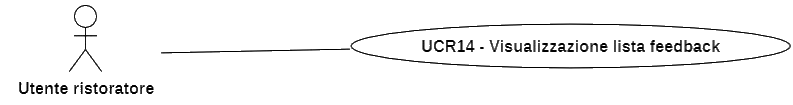
\includegraphics[width=0.8\textwidth]{./uml/UCR14.png} 
	\caption{Visualizzazione lista \textit{feedback}}
	\label{fig:UCR14}
\end{figure}

\begin{itemize}
	\item \textbf{Attore principale:} Utente ristoratore.

	\item \textbf{Precondizione:} L'Utente ristoratore ha effettuato l'accesso al sistema (vedi \autoref{usecase:Effettua accesso}).

	\item \textbf{Postcondizione:} L'Utente ristoratore visualizza la lista di \textit{feedback} inseriti da vari clienti.


	\item \textbf{Scenario principale:}
	      \begin{enumerate}
		      \item L'Utente ristoratore accede alla sezione dedicata alla 
				  visualizzazione del proprio ristorante;

		      \item Il Sistema mostra, tra le altre informazioni, la lista di \textit{feedback};

			  \item Per ogni \textit{feedback} il Sistema mostra:
				  \begin{itemize}
					  \item Il nome del cliente che ha inserito il \textit{feedback};
					  \item Il voto assegnato (da 1 a 10);
					  \item La descrizione del \textit{feedback};
					  \item La data di inserimento del \textit{feedback}.
				  \end{itemize}
	      \end{enumerate}
\end{itemize}
